\begin{frame}
\frametitle{Angle between planes}
\begin{columns}
\column{0.4\textwidth}
\psfrag{cP1}{$\mathcal{P}_2$}
\psfrag{cP2}{$\mathcal{P}_1$}
\psfrag{P1}{$P_2$}
\psfrag{P2}{$P_1$}
\psfrag{n1}{$\textbf{n}_2$}
\psfrag{n2}{$\textbf{n}_1$}
\psfrag{a}{$\alpha$}
\psfrag{u}{$\textbf{u}$}
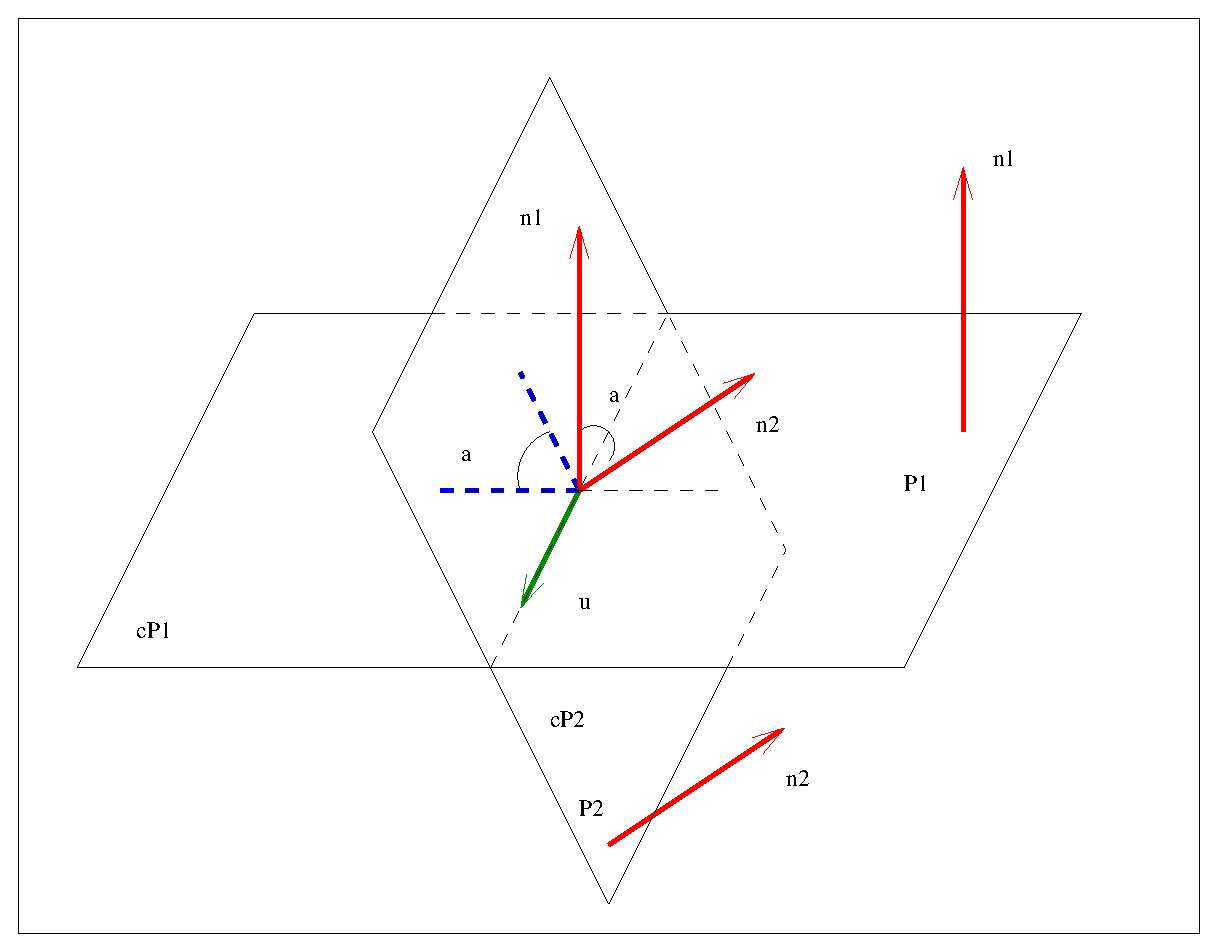
\includegraphics[height=1.3in]{../../modules/vectors/pictures/ok-angle_plane_plane.eps}
\column{0.6\textwidth}
\begin{itemize}
\item Given: planes $\mathcal{P}_1: \quad (\textbf{r} - \textbf{r}_1) \cdot \textbf{n}_1 = 0$, $\mathcal{P}_2: \quad (\textbf{r} - \textbf{r}_2) \cdot \textbf{n}_2 = 0$
\item Goal: find/define angle between the two planes.
\end{itemize}
\end{columns}
\alert<1->{Angle} $\alpha$ between planes:
\uncover<2->{
$
\begin{array}{rcl}
\alpha &=& \text{acute angle} (\textbf{n}_1,\textbf{n}_2) \\
\alpha &=&\arccos{\left( \frac{|\textbf{n}_1 \cdot \textbf{n}_2|}{|\textbf{n}_1|\, |\textbf{n}_2|}\right)}
\end{array}
$
}

\uncover<3->{\alert<1->{Perpendicular} planes:} \uncover<4->{$$\alpha = \frac{\pi}{2} \Longleftrightarrow \boxed{\textbf{n}_1 \cdot \textbf{n}_2 = 0}$$}
\uncover<5->{Direction of \textcolor[rgb]{0.98,0.00,0.00}{line of intersection}:}
\uncover<6->{$$\textbf{u} = \textbf{n}_1 \times \textbf{n}_2$$}
\end{frame}